\documentclass[tikz]{standalone}
\usepackage{amsmath}
\definecolor{bgcol}{HTML}{171D2B}
\definecolor{accent}{HTML}{F7B538}
\definecolor{setcol}{HTML}{7DA2C9}
\pagecolor{bgcol}
\begin{document}

% Gambar 1: kurva y = 240/x dengan titik-titik dari tabel
% pekerja 6->40, 8->30, 10->24, 12->20, 15->16, 16->15, 20->12, 24->10, 30->8
% semua hasil kali = 240 pekerja-hari
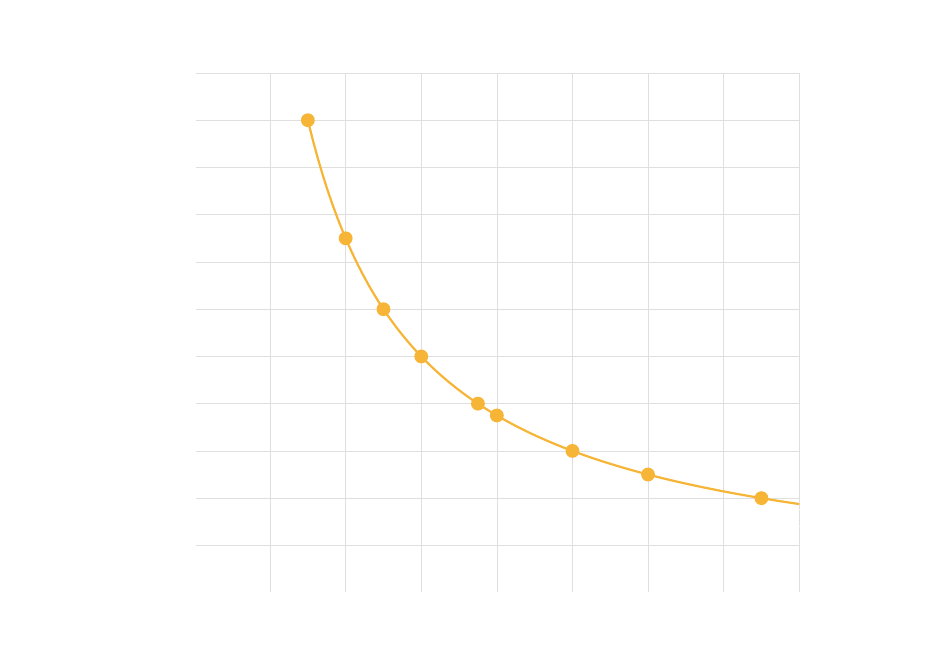
\begin{tikzpicture}[x=0.24cm, y=0.15cm, color=white, font=\small]
  % Kisi tipis setiap 4 satuan
  \draw[step=4, gray!25, very thin] (0, 0) grid (32, 44);
  % Sumbu
  \draw[->, thick] (0, 0) -- (33, 0) node[below] {Banyak pekerja};
  \draw[->, thick] (0, 0) -- (0, 46) node[left] {Waktu (hari)};
  % Tanda skala sumbu
  \foreach \x in {8, 16, 24, 32}
    \node[below] at (\x, 0) {$\x$};
  \foreach \y in {8, 16, 24, 32, 40}
    \node[left] at (0, \y) {$\y$};
  % Kurva y = 240/x
  \draw[thick, accent] plot[domain=6:32, samples=100] (\x, {240/\x});
  % Titik-titik dari tabel
  \foreach \x/\y in {6/40, 8/30, 10/24, 12/20,
    15/16, 16/15, 20/12, 24/10, 30/8}
    \fill[accent] (\x, \y) circle (2.5pt);
  % Label dua titik ujung
  \node[above] at (6, 40) {$(6, 40)$};
  \node[below right] at (30, 8) {$(30, 8)$};
\end{tikzpicture}

% Gambar 2: kurva benar vs garis lurus yang menipu
% Garis lurus (6,40)-(30,8): kemiringan -4/3, pada x=12 nilainya 32 (salah)
% Kurva pada x=12 nilainya 20 (benar)
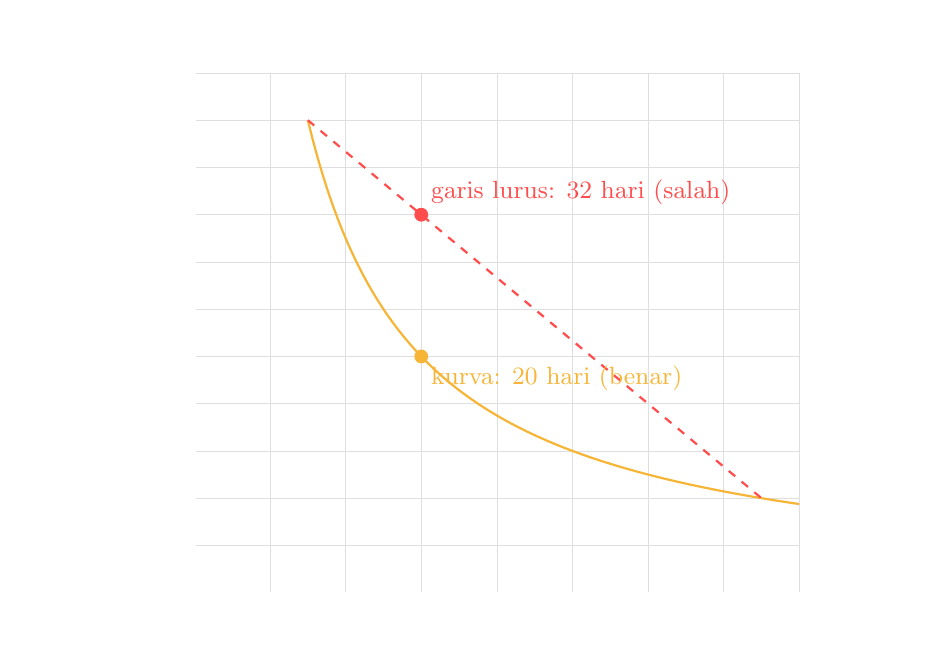
\begin{tikzpicture}[x=0.24cm, y=0.15cm, color=white, font=\small]
  % Kisi tipis setiap 4 satuan
  \draw[step=4, gray!25, very thin] (0, 0) grid (32, 44);
  % Sumbu
  \draw[->, thick] (0, 0) -- (33, 0) node[below] {Banyak pekerja};
  \draw[->, thick] (0, 0) -- (0, 46) node[left] {Waktu (hari)};
  % Tanda skala sumbu
  \foreach \x in {8, 16, 24, 32}
    \node[below] at (\x, 0) {$\x$};
  \foreach \y in {8, 16, 24, 32, 40}
    \node[left] at (0, \y) {$\y$};
  % Kurva y = 240/x (benar)
  \draw[thick, accent] plot[domain=6:32, samples=100] (\x, {240/\x});
  % Garis lurus yang SALAH, dari (6,40) ke (30,8)
  \draw[dashed, red!70, thick] (6, 40) -- (30, 8);
  % Titik pada x = 12: kurva benar, garis lurus salah
  \fill[accent] (12, 20) circle (2.5pt);
  \fill[red!70] (12, 32) circle (2.5pt);
  \node[below right, accent] at (12, 20) {kurva: 20 hari (benar)};
  \node[above right, red!70] at (12, 32) {garis lurus: 32 hari (salah)};
\end{tikzpicture}

\end{document}
